%%%%%
%Soubor: proj5.tex
%Datum: 28.04.2012
%Autor: Jan Wrona, xwrona00@stud.fit.vutbr.cz
%Projekt: Projekt c. 5 pro predmet ITY
%%%%%

\documentclass[pdf, frames]{prosper}[28.04.2012]
  \usepackage[czech]{babel}
  \usepackage[utf8]{inputenc}
  \usepackage[T1]{fontenc}
  \usepackage{multirow}
  \usepackage{colortbl}

  \title{Typografie a publikování\\ \quad ITY 2011/2012}
  \subtitle{Projekt č. 5}
  \author{Jan Wrona}
  \email{xwrona00@stud.fit.vutbr.cz}
  \institution{Vysoké učetní technické v Brně}
  \displayVersion

  \ptsize{12}
  \FontText{\fontsize{12pt}{12pt}\selectfont}{\black\fontsize{12pt}{12pt}\selectfont}

\begin{document}
\maketitle
\overlays{2}{
\begin{slide}{Návrh počítačové sestavy}
  V této prezentaci se věnuji popisu návrhu počítačové sestavy, včetně specifikace požadavků, 
  výpisu součástek, zhodnocení kladů a záporů a finálnímu cenovému návrhu.

  \bigskip
  \FromSlide{2}
  Specifikace požadavků:
  \begin{itemize}
    \item Vysoký výkon 3D akcelerátoru
    \item Tichý chod, nízká spotřeba v idle
    \item Rychlý start systému
    \item \bf{Cena: 25\,000 -- 30\,000 Kč}
  \end{itemize}
  \end{slide}
}

\begin{slide}[Dissolve]{Soupis součástek}
  \begin{table}
  \catcode`\-=12
  \begin{tabular}{|l|l|l|}
    \hline
    \rowcolor[gray]{0.5}
    Součástka & Model & Cena [Kč]\\ \hline
    Základní deska & ASUS P8Z68-V LX & 2\,499\\ \hline
    Procesor & Intel Core i5-2500K & 4\,885\\ \hline
    Grafická karta & Radeon HD 7850 & 5\,615\\ \hline
    Paměti RAM & Kingston HyperX 2x4\,GB & 1\,199\\ \hline
    \multirow{2}{*}{Pevné disky} & WD Caviar Green 2\,TB & 2\,690 \\ \cline{2-3}
     & OCZ Agility 3 Series 120\,GB & 3\,152\\ \hline
    Blu-ray mechanika & Lite-On iHOS104 & 1\,431 \\ \hline
    PC skříň & Lian Li PC-60FN & 2\,350\\ \hline
    PC zdroj & Seasonic X-760 760W & 3\,675\\ \hline
  \end{tabular}
  \caption{Soupis součástek}
  \end{table}
\end{slide}

\overlays{2}{
\begin{slide}{Detailní pohled na GPU}
  Klíčové parametry:
  \begin{itemize}
    \item Frekvence: paměti 1\,200\,MHz, jádro 860\,MHz
    \item Pamět: 2\,GB technologie GDDR5
  \end{itemize}

  Využité technologie:
  \begin{itemize}
    \item PCI Express 3.0 x16
    \item DirectX \copyright 11.1
    \item OpenGL 4.2
  \end{itemize}
  \FromSlide{2}
  \vspace{-2cm}
  \flushright
  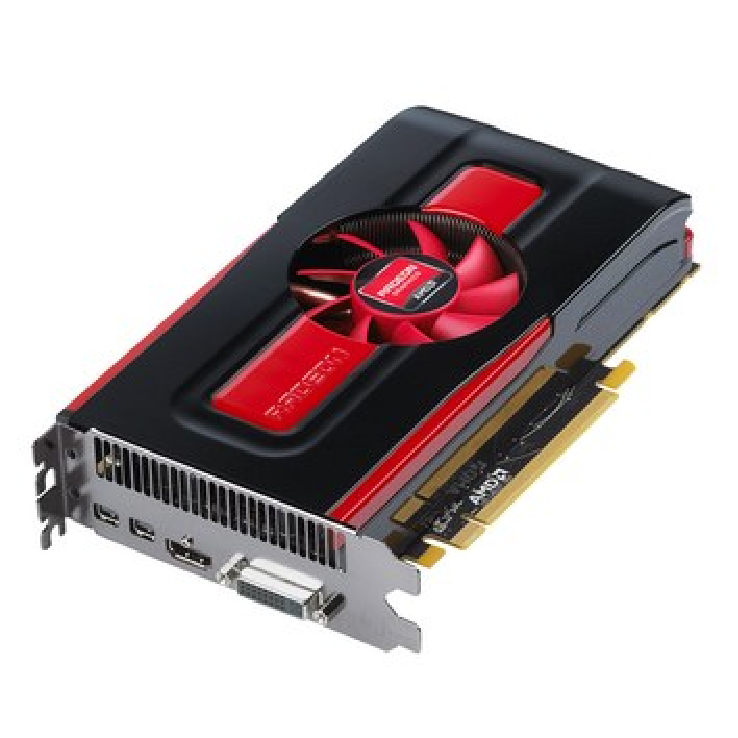
\includegraphics[width=5cm]{gpu.eps}
\end{slide}
}

\begin{slide}{Nákres PC skříně}
  \begin{figure}
  \centering
  \setlength{\unitlength}{0.6mm}
  \begin{picture}(50, 83.5)
    \put(0, 0){\line(0, 1){47.5}}
    \put(21, 0){\line(0, 1){47.5}}
    \put(0, 0){\line(1, 0){21}}
    \put(0, 47.5){\line(1, 0){21}}
    \put(21, 0){\line(1, 2){18}}
    \put(21, 47.5){\line(1, 2){18}}
    \put(0, 47.5){\line(1, 2){18}}
    \put(39, 36){\line(0, 1){47}}
    \put(18, 83.5){\line(1, 0){21}}
    \multiput(0, 47.5)(0, -7){4}{\line(1, 0){21}}
    \put(10.5, 10.5){\circle{17}}
  \end{picture}
  \begin{picture}(45, 50)
    \put(0, 0){\line(0, 1){47.5}}
    \put(21, 0){\line(0, 1){47.5}}
    \put(0, 0){\line(1, 0){21}}
    \put(0, 47.5){\line(1, 0){21}}
    \multiput(0, 47.5)(0, -7){4}{\line(1, 0){21}}
    \put(10.5, 10.5){\circle{17}}
    \put(0, -1){\line(0, -1){6}}
    \put(21, -1){\line(0, -1){6}}
    \put(0, -7){\vector(1, 0){21}}
    \put(0, -7){\vector(-1, 0){0}}
    \put(6, -6.5){210}
    \put(22, 0){\line(1,  0){6}}
    \put(22, 47.5){\line(1,  0){6}}
    \put(28, 0){\vector(0, 1){47.5}}
    \put(28, 0){\vector(0, -1){0}}
    \put(29, 23){475}
  \end{picture}
  \begin{picture}(60, 60)
    \put(0, 0){\line(1, 0){50}}
    \put(0, 47.5){\line(1, 0){50}}
    \put(0, 0){\line(0, 1){47.5}}
    \put(50, 0){\line(0, 1){47.5}}

    \put(0, -1){\line(0, -1){6}}
    \put(50, -1){\line(0, -1){6}}
    \put(0, -7){\vector(1, 0){50}}
    \put(0, -7){\vector(-1, 0){0}}
    \put(20, -6.5){500}
    \put(51, 0){\line(1,  0){6}}
    \put(51, 47.5){\line(1,  0){6}}
    \put(57, 0){\vector(0, 1){47.5}}
    \put(57, 0){\vector(0, -1){0}}
    \put(58, 23){475}
  \end{picture}

  \caption{Technický nákres PC skříně}
  \end{figure}
\end{slide}

\overlays{5}{
\begin{slide}{Zhodnocení}
  \begin{itemstep}
    \item Tichý chod zajištěn díky kvalitní PC skříni
    \item Vysoký 3D výkon zajištěn výkonným grafickým adaptérem
    \item Nízká spotřeba zajištěna technologiemi na základní desce, především přepínáním integrovaného
    a dedikovaného grafického adaptéru
    \item Rychlý start systému zajištěn pomocí SSD
  \end{itemstep}
  \FromSlide{5}
  \medskip
  \begin{itemize}
    \item \bf{Celková cena: 27\,802\,Kč}
  \end{itemize}
\end{slide}
}

\end{document}
